
\documentclass[11pt,a4paper,UTF8]{book}

\usepackage[T1]{fontenc}
\usepackage[utf8]{inputenc}
\usepackage{authblk}
\usepackage{amssymb}

\usepackage{fontspec}                  %引入字体设置宏包
\setmainfont{Times New Roman}             %设置英文正文字体
% Courier New
% Book Antique
\setsansfont{Arial}                    %英文无衬线字体
\setmonofont{Courier New}              %英文等宽字体

\usepackage{ctex} %导入中文包
%\usepackage{ulem}
\usepackage{tocvsec2}
\usepackage{verbatim}

\usepackage{tabularx}
\usepackage{booktabs} 
\usepackage{multirow}
\usepackage{bbding}
\usepackage{float}
\usepackage{xspace}
\usepackage[none]{hyphenat}

\usepackage{graphicx}
\usepackage{subfigure}
\usepackage{pifont}

\usepackage{hyperref}  %制作pdf的目录
\usepackage{subfiles} %使用多文件方式进行

\usepackage{geometry} %设置页边距的包
\geometry{left=2.5cm,right=2cm,top=2.54cm,bottom=2.54cm} %设置书籍的页边距

\usepackage{url}
\hypersetup{hidelinks, %去红框
	colorlinks=true,
	allcolors=black,
	pdfstartview=Fit,
	breaklinks=true
}

% 调整itemlist中的行间距
\usepackage{enumitem}
\setenumerate[1]{itemsep=0pt,partopsep=0pt,parsep=\parskip,topsep=5pt}
\setitemize[1]{itemsep=0pt,partopsep=0pt,parsep=\parskip,topsep=5pt}
\setdescription{itemsep=0pt,partopsep=0pt,parsep=\parskip,topsep=5pt}

% 超链接样式设置
\usepackage{hyperref}
\hypersetup{
	colorlinks=true,
	linkcolor=blue,
	filecolor=blue,
	urlcolor=blue,
	citecolor=cyan,
}

\usepackage{indentfirst}

\usepackage{listings}
\usepackage[usenames,dvipsnames,svgnames, x11names, table, xcdraw]{xcolor}

\usepackage[most]{tcolorbox}

%展示代码
\definecolor{mygreen}{rgb}{0,0.6,0}
\definecolor{mygray}{rgb}{0.5,0.5,0.5}
\definecolor{mymauve}{rgb}{0.58,0,0.82}
\definecolor{keywordcolor}{rgb}{0.8,0.1,0.5}
\definecolor{webgreen}{rgb}{0,.5,0}
\definecolor{bgcolor}{rgb}{0.92,0.92,0.92}

%定义CMake
\lstdefinelanguage{CMake}
{morekeywords={
		cmake\_minimum\_required,
		project,
		add\_executable,
		add\_library,
		target\_link\_libraries,
		cmake\_parse\_arguments,
		cmake\_language,
		set, unset,
		option,
		string,
		list,
		math,
		message,
		if, elseif, else, endif,
		mark\_as\_advanced,
		foreach, endforeach,
		while, endwhile,
		add\_subdirectory, include, return, include\_gurad,
		function, endfunction,
		macro, endmacro,
		find\_package,
		cmake\_push\_check\_state,
		cmake\_pop\_check\_state,
		cmake\_reset\_check\_state,
		add\_test,
		set\_tests\_properties, 
		check\_c\_source\_runs,
		check\_cxx\_source\_runs,
		check\_fortran\_source\_runs,
		check\_source\_runs,
		check\_compiler\_flag,
		check\_c\_compiler\_flag,
		check\_cxx\_compiler\_flag,
		check\_fortran\_compiler\_flag,
		check\_symbol\_exists,
		check\_cxx\_symbol\_exists,
		check\_linker\_flag,
		cmake\_policy,
		set\_property,
		get\_property,
		define\_property,
		get\_cmake\_property,
		set\_cmake\_property,
		set\_target\_properties,
		get\_target\_property,
		set\_directory\_properties,
		get\_directory\_property,
		set\_source\_files\_properties,
		get\_source\_file\_property,
		set\_tests\_properties,
		get\_tests\_property,
		get\_test\_property,
		cmake\_print\_properties,
		cmake\_print\_variables,
		variable\_watch,
		include\_guard,
		target\_link\_options,
		target\_compile\_definitions,
		target\_compile\_options,
		include\_directories,
		add\_definitions,
		remove\_definitions,
		add\_compile\_definitions,
		add\_compile\_options,
		link\_libraries,
		link\_directories,
		add\_link\_options,
		target\_include\_directories,
		target\_compile\_features,
		add\_custom\_command,
		add\_custom\_target,
		execute\_process,
		cmake\_path,
		get\_filename\_component,
		file,
		configure\_file,
		generate\_export\_header,
		export,
		find\_file,
		find\_library,
		find\_package,
		find\_program,
		pkg\_check\_modules,
		pkg\_search\_module,
		pkg\_get\_variable,
		add\_test,
		enable\_testing,
		set\_tests\_properties,
		site\_name,
		ctest\_empty\_binary\_directory,
		ctest\_start,
		ctest\_configure,
		ctest\_submit,
		ctest\_build,
		ctest\_memcheck,
		ctest\_upload,
		ctest\_test,
		gtest\_add\_tests,
		gtest\_discover\_tests,
		install,
		write\_basic\_package\_version\_file,
		configure\_package\_config\_file,
		cpack\_add\_component,
		cpack\_add\_install\_type,
		cpack\_add\_component\_group,
		ExternalProject\_Add,
		ExternalProject\_Add\_StepDependencies,
		ExternalProject\_Get\_Property,
		ExternalProject\_Add\_Step,
		FetchContent\_Declare,
		FetchContent\_GetProperties,
		FetchContent\_Populate,
		source\_group,
		target\_precompile\_headers,
		qt5\_wrap\_cpp,
		qt5\_wrap\_ui,
		qt5\_add\_resources,
		qt5\_add\_big\_resources,
		qt5\_add\_binary\_resources,
		qt5\_add\_translation,
		qt5\_create\_translation,
		compile\_definitions,
		add\_llvm\_component\_library,
		add\_llvm\_tool,
		llvm\_multisource,
		llvm\_test\_data,
		doxygen\_add\_docs,
	}, %定义关键字
	sensitive=false, %是否大小写敏感
	morecomment=[l]{\#},
	morestring=[b]",
	morestring=[d]',
}

\lstdefinestyle{styleCXX}{
	language = C++,  
	backgroundcolor=\color{blue!3!white}, 
	%basicstyle = \footnotesize,  
	basicstyle      =   \zihao{-5}\ttfamily,
	numberstyle     =   \zihao{-5}\ttfamily,   
	%breakatwhitespace = false,    
	basewidth       =   0.5em,    
	breaklines = true,                 
	captionpos = b,                    
	commentstyle = \color{mygray}\bfseries,
	%extendedchars = false,             
	frame =shadowbox, 
	framerule=0.5pt,
	%frameround = fttt,
	keepspaces=true,
	keywordstyle=\color{blue}\bfseries, % keyword style
	otherkeywords={string}, 
	numbers=left, 
	numbersep=5pt,
	numberstyle=\tiny\color{mygray},
	rulecolor=\color{black},         
	%showspaces=false,  
	%showstringspaces=false, 
	%showtabs=false,    
	%stepnumber=1,         
	stringstyle=\color{mymauve},        % string literal style
	tabsize=2,          
	columns         =   fixed,
	flexiblecolumns,                   
}


\lstdefinestyle{styleCMake}{
	language=CMake,
	backgroundcolor=\color{blue!3!white}, 
	basicstyle=\tt, 
	breakatwhitespace = false,
	breaklines = true,
	captionpos = b,
	commentstyle = \color{mygray}\bfseries, 
	extendedchars =false,             
	frame=shadowbox, 
	tabsize=2,
	framerule=0.5pt,
	keepspaces=true,
	keywordstyle=\color{blue}\bfseries, % keyword style
	otherkeywords={string}, 
	rulecolor=\color{black},
	showspaces=false,
	showstringspaces=false,
	showtabs=false,
	stepnumber=1,
	stringstyle=\color{purple},        % string literal style
}

\lstdefinestyle{stylePython}{
	language        =   Python, % 语言选Python
	backgroundcolor=\color{blue!3!white}, 
	basicstyle      =   \zihao{-5}\ttfamily,
	numberstyle     =   \zihao{-5}\ttfamily,
	keywordstyle    =   \color{blue},
	keywordstyle    =   [2] \color{teal},
	stringstyle     =   \color{magenta},
	commentstyle    =   \color{red}\ttfamily,
	frame = shadowbox, 
	breaklines      =   true,   % 自动换行,建议不要写太长的行
	columns         =   fixed,  % 如果不加这一句,字间距就不固定,很丑,必须加
	basewidth       =   0.5em,
	%basicstyle          =   \sffamily,          % 基本代码风格
	%keywordstyle        =   \bfseries,          % 关键字风格
	%commentstyle        =   \rmfamily\itshape,  % 注释的风格,斜体
	%stringstyle         =   \ttfamily,  % 字符串风格
	flexiblecolumns,                % 别问为什么,加上这个
	%numbers             =   left,   % 行号的位置在左边
	showspaces          =   false,  % 是否显示空格,显示了有点乱,所以不现实了
	numberstyle         =   \zihao{-5}\ttfamily,    % 行号的样式,小五号,tt等宽字体
	showstringspaces    =   false,
	captionpos          =   t,      % 这段代码的名字所呈现的位置,t指的是top上面
	frame               =   lrtb,   % 显示边框
	tabsize=2,  
}

\tcbset{
	commandshell/.style={
		listing only,
		colback=black!75!white,
		colupper=white,
		lowerbox=ignored,
		listing options={
			language={bash},
			basicstyle=\ttfamily,
			columns = fixed,
			flexiblecolumns
		}
}}

\usepackage{tikz}
\usetikzlibrary{chains,scopes,positioning,backgrounds,shapes,fit,shadows,calc,arrows.meta,decorations.pathreplacing,calligraphy}

\newcommand{\mybrace}[4]{ \draw[#4, decoration={brace, amplitude=6}, decorate] ([yshift=3mm]#1)--([yshift=3mm]#2) node[midway, above=2mm]{#3}; }

% URL 正确换行
% https://liam.page/2017/05/17/help-the-url-command-from-hyperref-to-break-at-line-wrapping-point/
\makeatletter
\def\UrlAlphabet{%
	\do\a\do\b\do\c\do\d\do\e\do\f\do\g\do\h\do\i\do\j%
	\do\k\do\l\do\m\do\n\do\o\do\p\do\q\do\r\do\s\do\t%
	\do\u\do\v\do\w\do\x\do\y\do\z\do\A\do\B\do\C\do\D%
	\do\E\do\F\do\G\do\H\do\I\do\J\do\K\do\L\do\M\do\N%
	\do\O\do\P\do\Q\do\R\do\S\do\T\do\U\do\V\do\W\do\X%
	\do\Y\do\Z}
\def\UrlDigits{\do\1\do\2\do\3\do\4\do\5\do\6\do\7\do\8\do\9\do\0}
\g@addto@macro{\UrlBreaks}{\UrlOrds}
\g@addto@macro{\UrlBreaks}{\UrlAlphabet}
\g@addto@macro{\UrlBreaks}{\UrlDigits}
\makeatother

% enable subsubsubsection
% from https://tex.stackexchange.com/questions/274212/correct-hierarchy-levels-of-pdf-bookmarks-for-custom-section-subsubsubsection
\usepackage[depth=3]{bookmark}
\setcounter{secnumdepth}{3}
\setcounter{tocdepth}{4}
\hypersetup{bookmarksdepth=4}

\makeatletter

\newcommand{\toclevel@subsubsubsection}{4}
\newcounter{subsubsubsection}[subsubsection]

\renewcommand{\thesubsubsubsection}{\thesubsubsection.\arabic{subsubsubsection}}

\newcommand{\subsubsubsection}{\@startsection{subsubsubsection}{4}{\z@}%
	{-3.25ex\@plus -1ex \@minus -.2ex}%
	{1.5ex \@plus .2ex}%
	{\normalfont\normalsize\bf\bfseries}}

\newcommand*{\l@subsubsubsection}{\@dottedtocline{4}{11em}{5em}}  

\newcommand{\subsubsubsectionmark}[1]{}
\makeatother

\begin{document}
\begin{sloppypar} %latex中一行文字出现溢出问题的解决方法
	%\maketitle
	
	\begin{center}
		\thispagestyle{empty}
		%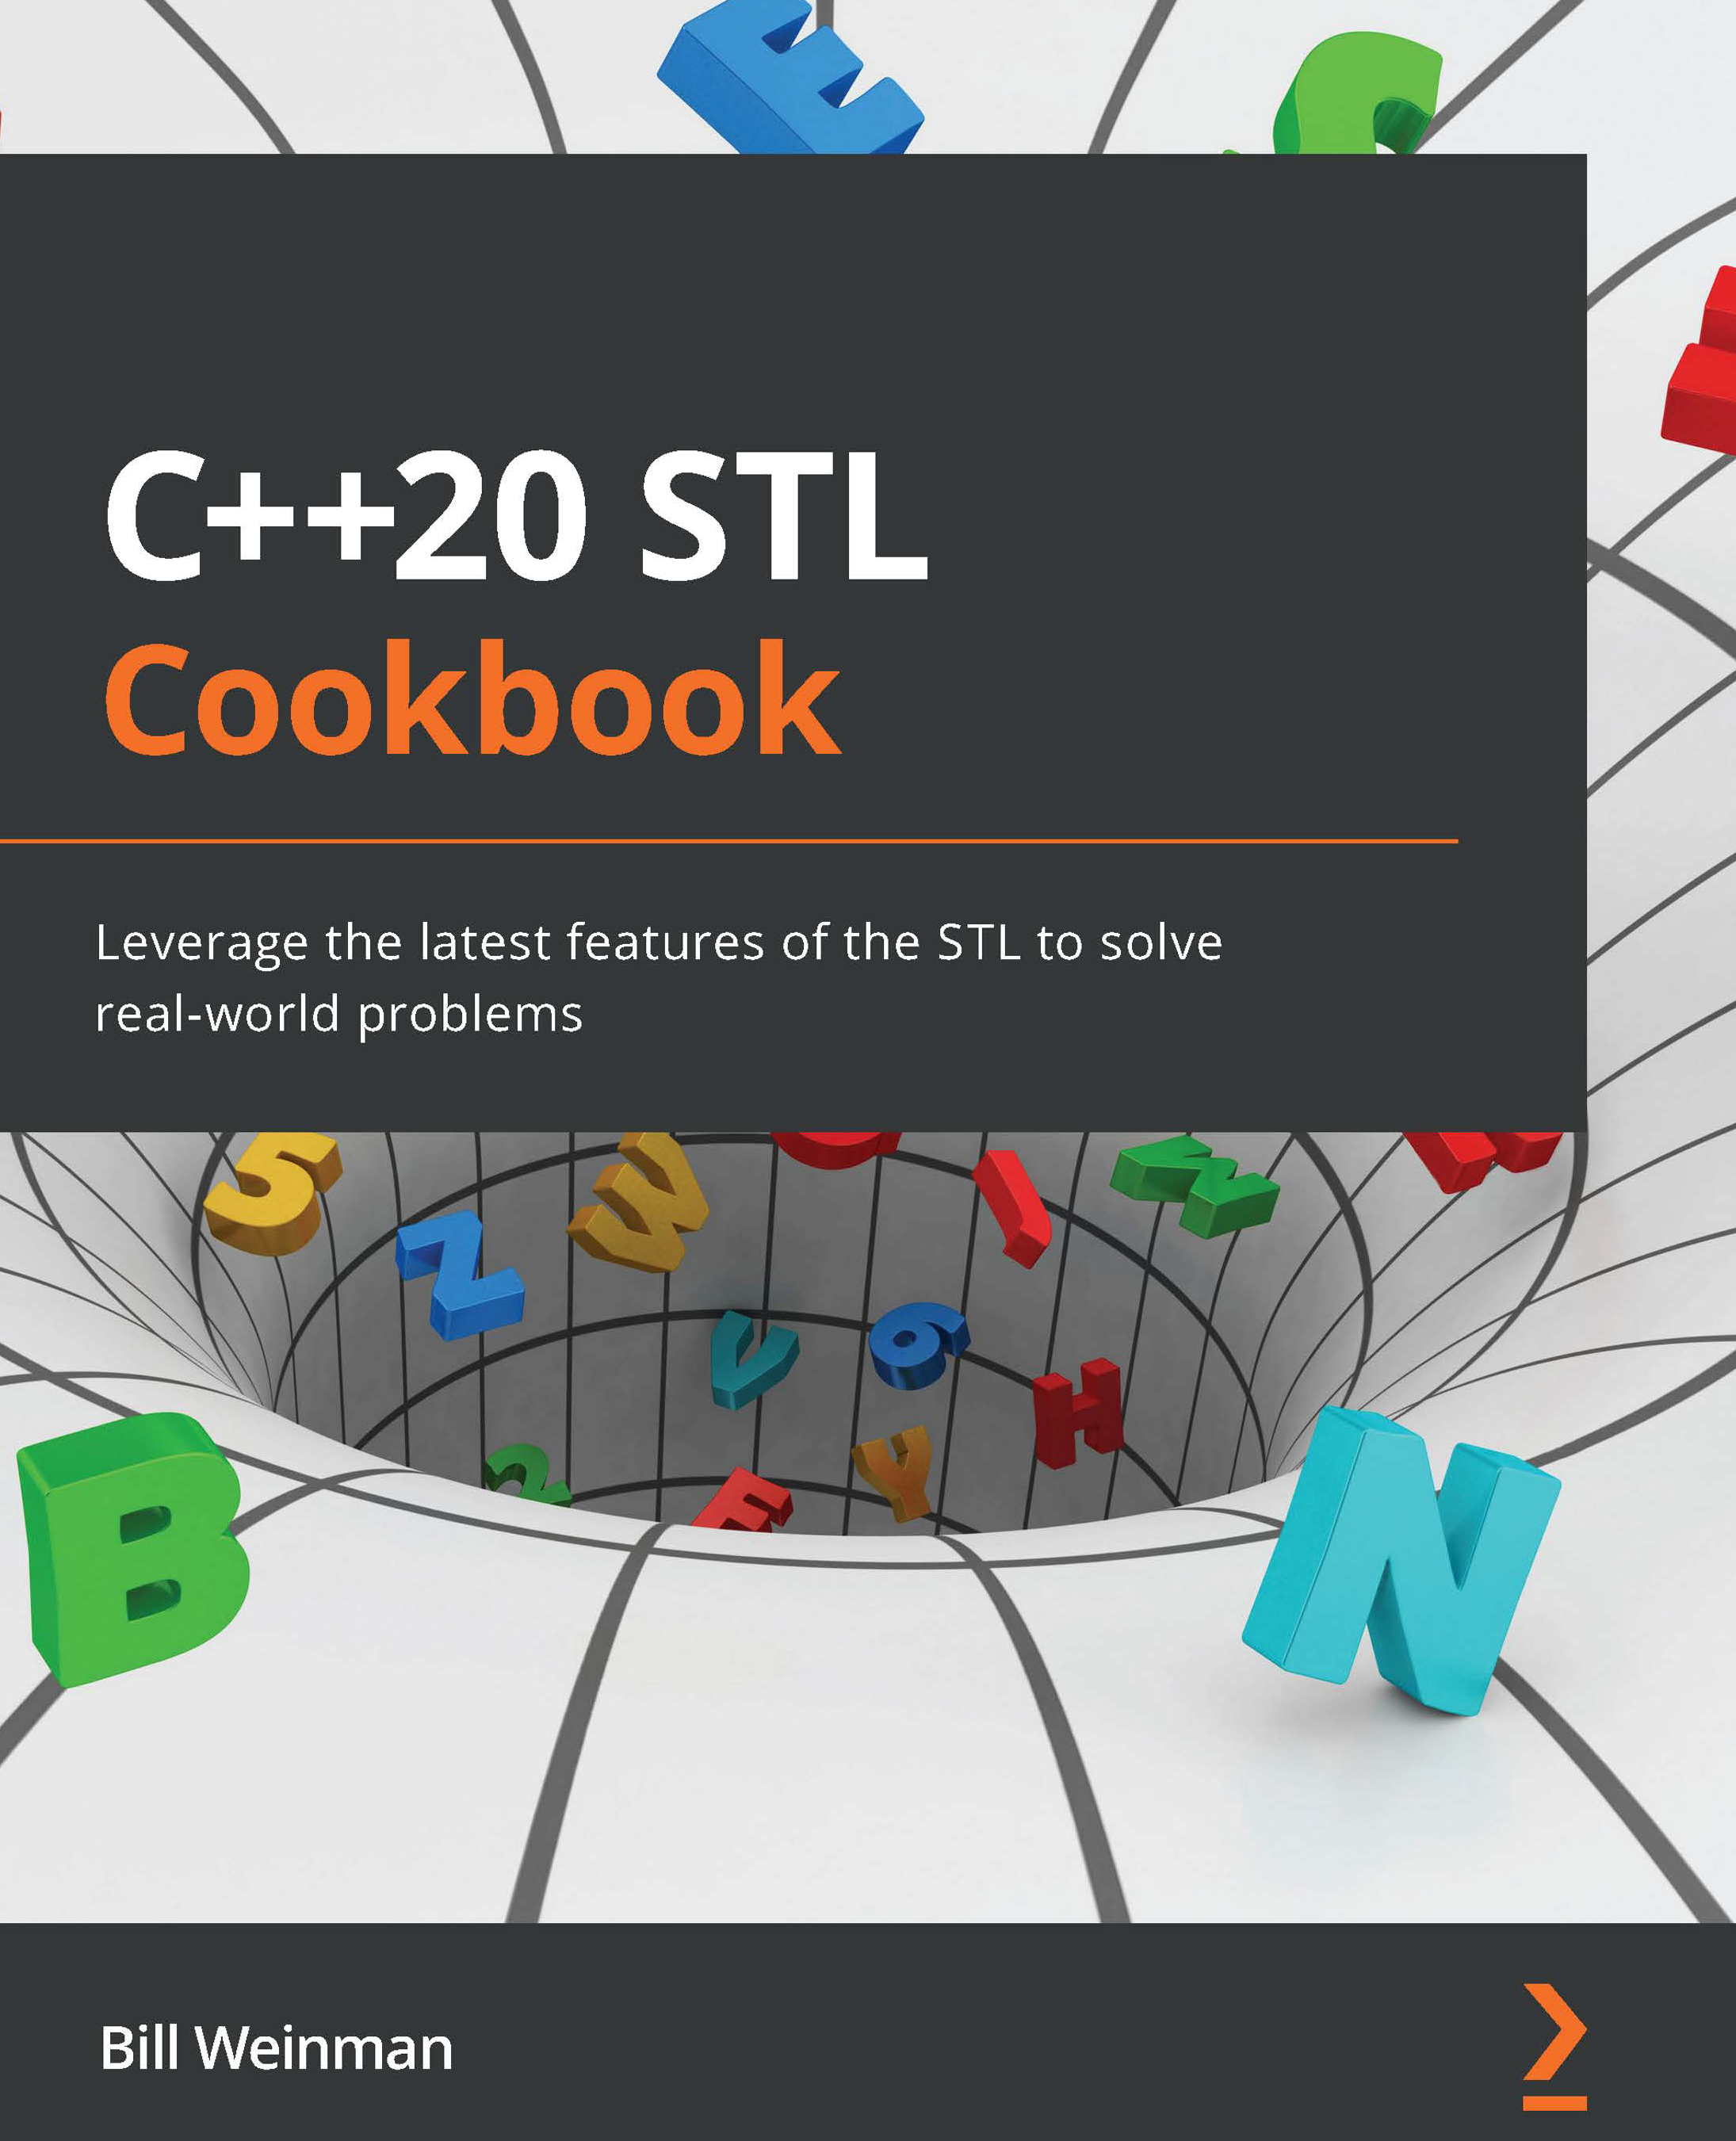
\includegraphics[width=\textwidth,height=\textheight,keepaspectratio]{cover.jpg}
		\begin{tikzpicture}[remember picture, overlay, inner sep=0pt]
			\node at (current page.center) 
			{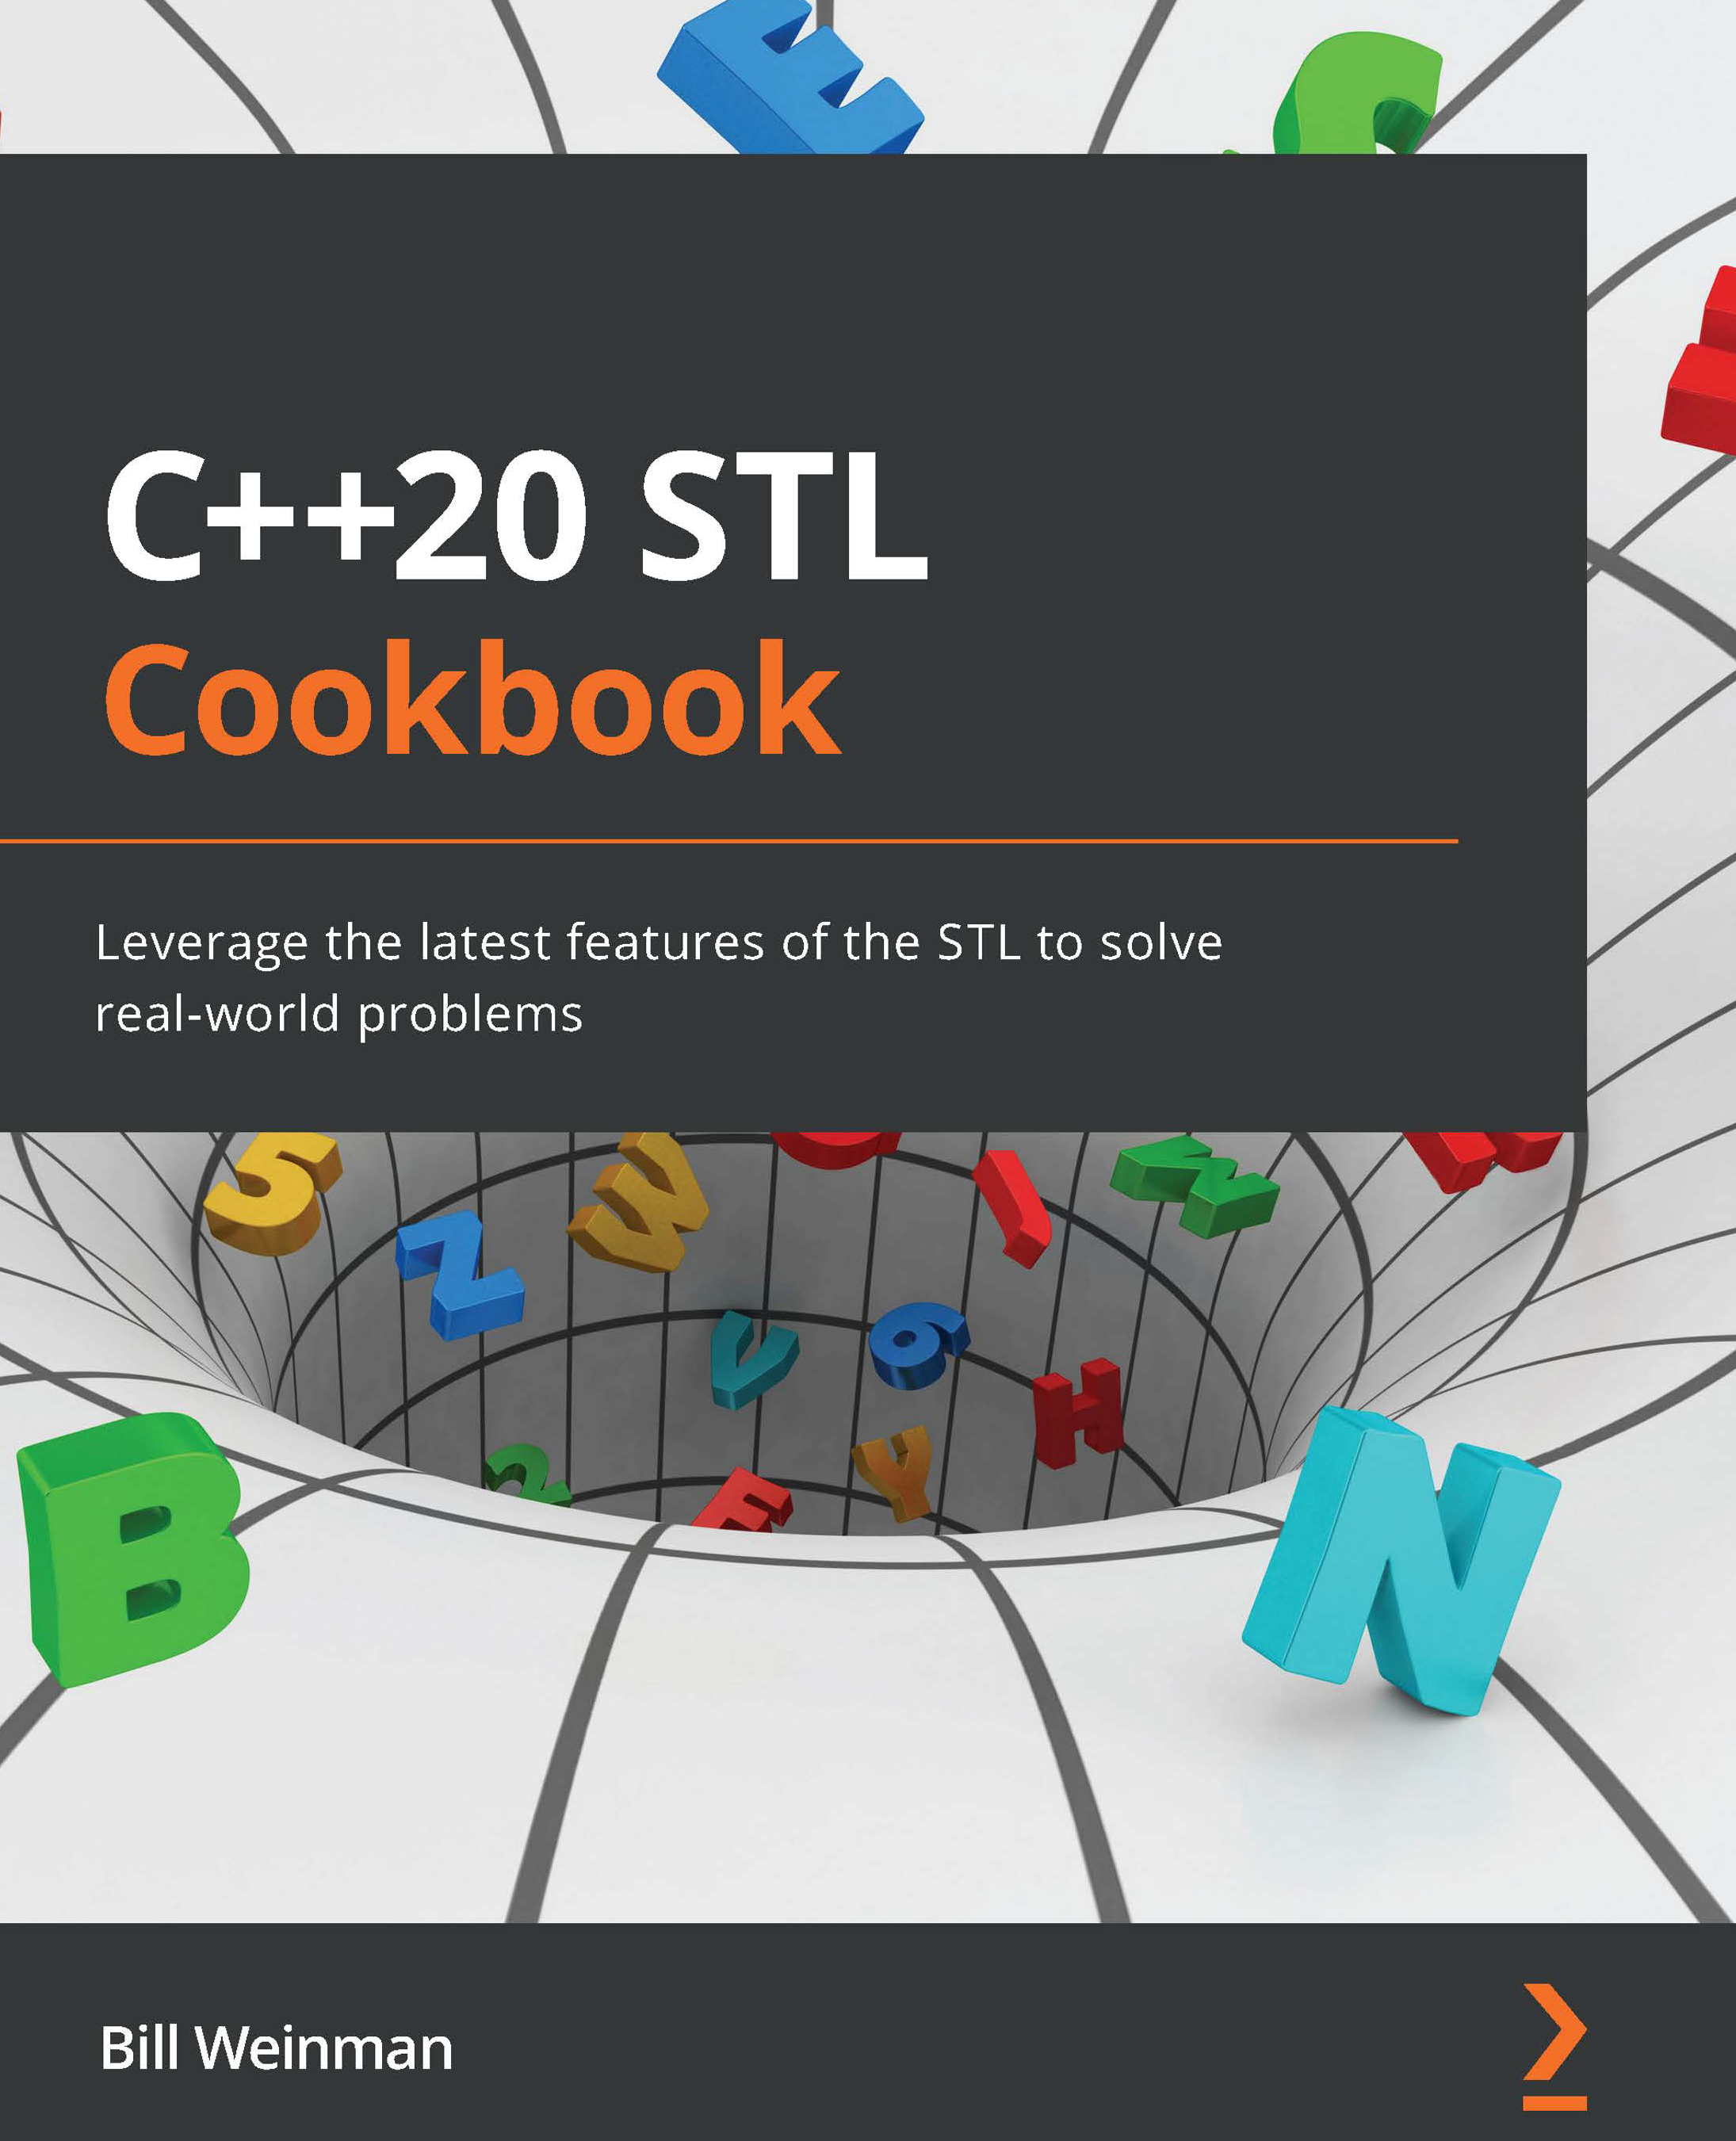
\includegraphics[width=\paperwidth, keepaspectratio=false]{cover.png}};
		\end{tikzpicture}
		\newpage
		\thispagestyle{empty}
		\huge
		\textbf{C++20 STL Cookbook} 
		\\[9pt]
		\normalsize
		Leverage the latest features of the STL to solve real-world problems
		\\[9pt]
		\normalsize
		使用STL的新特性来解决实际问题
		\\[10pt]
		\normalsize 
		作者: Bill Weinman 
		\\[8pt]
		\normalsize
		译者:陈晓伟
	\end{center}
	
	\hspace*{\fill} \\ %插入空行
	\noindent\textbf{本书概述}
	
	快速、高效和灵活是C++编程语言一直以来的特点,从而应用于行业的各个领域来解决许多问题。最新版本的C++ 20将改变开发者的编码方式,因为它带来了一系列支持应用程序快速部署的特性。这本书将帮助您以最优的方式使用STL。
	
	本书将从C++ 20中的新语言特性开始,帮助您理解该语言的机制和库特性,并了解它们是如何工作的。与其他书籍不同,C++ 20 STL Cookbook采用了一种特定于实现的问题解决方法,将帮助您快速克服障碍。您将学习核心STL概念,如容器、算法、实用程序类、Lambda表达式、迭代器等,学习的同时结合实践。本书是使用C++ STL及其最新功能的参考指南,可用来探索函数式编程和Lambda表达式中的前沿特性。
	
	阅读完这本书后,您将能够利用最新的C++特性,并节省时间和精力,同时可以优雅地使用STL解决实际问题。
	
	\hspace*{\fill} \\ %插入空行
	\noindent\textbf{关键特性}
	\begin{itemize}
		\item 熟悉C++ 20的最新特性,并使用STL编写更好的代码
		\item 减少应用的开发时间,并支持更快的部署
		\item 启动和使用新版本中引入的、更精简的STL功能
	\end{itemize}
	
	\hspace*{\fill} \\ %插入空行
	\noindent\textbf{作者简介}
	
	\textbf{Bill Weinman}自从他在1971年16岁时拥有了他的第一台计算机以来,他一直在从事技术工作。自20世纪70年代初以来,一直用C和C++编程,为包括NASA、美国银行、施乐、IBM和美国海军在内的主要客户编写系统和应用程序。他还是一名电子工程师,曾为旅行者II号宇宙飞船、SAE的音频放大器和Altec Lansing的音响系统工作。
	
	自20世纪90年代中期以来,Weinman先生一直专注于写作和教学。他的书和课程涵盖了HTML、SQL、CGI、Python,当然还有C和C++。作为在线学习的早期贡献者,清晰、简洁的授课方式使他的课程在lynda和LinkedIn learning上很受欢迎。
	
	可以关注Bill的网站:bw.org。
	。
	
	\hspace*{\fill} \\ %插入空行
	\noindent\textbf{本书相关}
	\begin{itemize}
		\item Github地址:\\\url{https://github.com/xiaoweiChen/CXX20-STL-Cookbook}
	\end{itemize}
	\newpage
	
	%前言
	\pagestyle{empty}
	\subfile{content/preface.tex}
	\newpage
	
	\tableofcontents
	\newpage

	\setsecnumdepth{section}

	\section*{\zihao{2} 第1章\hspace{0.5cm}New C++20 Features}
	\addcontentsline{toc}{section}{第1章\hspace{0.5cm}New C++20 Features}
	\subfile{content/chapter1/0.tex}
	
	\subsection*{\zihao{3} 1.1.\hspace{0.2cm}Technical requirements}
	\addcontentsline{toc}{subsection}{1.1.\hspace{0.2cm}Technical requirements}
	\subfile{content/chapter1/1.tex}
	
	\subsection*{\zihao{3} 1.2.\hspace{0.2cm}Format text with the new format library}
	\addcontentsline{toc}{subsection}{1.2.\hspace{0.2cm}Format text with the new format library}
	\subfile{content/chapter1/2.tex}
	
	\subsection*{\zihao{3} 1.3.\hspace{0.2cm}Use compile-time vectors and strings with constexpr}
	\addcontentsline{toc}{subsection}{1.3.\hspace{0.2cm}Use compile-time vectors and strings with constexpr}
	\subfile{content/chapter1/3.tex}
	
	\subsection*{\zihao{3} 1.4.\hspace{0.2cm}Safely compare integers of different types}
	\addcontentsline{toc}{subsection}{1.4.\hspace{0.2cm}Safely compare integers of different types}
	\subfile{content/chapter1/4.tex}
	
	\subsection*{\zihao{3} 1.5.\hspace{0.2cm}Use the "spaceship" operator <=> for threeway comparisons}
	\addcontentsline{toc}{subsection}{1.5.\hspace{0.2cm}Use the "spaceship" operator <=> for threeway comparisons}
	\subfile{content/chapter1/5.tex}
	
	\subsection*{\zihao{3} 1.6.\hspace{0.2cm}Easily find feature test macros with the <version> header}
	\addcontentsline{toc}{subsection}{1.6.\hspace{0.2cm}Easily find feature test macros with the <version> header}
	\subfile{content/chapter1/6.tex}
	
	\subsection*{\zihao{3} 1.7.\hspace{0.2cm}Create safer templates with concepts and constraints}
	\addcontentsline{toc}{subsection}{1.7.\hspace{0.2cm}Create safer templates with concepts and constraints}
	\subfile{content/chapter1/7.tex}
	
	\subsection*{\zihao{3} 1.8.\hspace{0.2cm}Avoid re-compiling template libraries with modules}
	\addcontentsline{toc}{subsection}{1.8.\hspace{0.2cm}Avoid re-compiling template libraries with modules}
	\subfile{content/chapter1/8.tex}
	
	\subsection*{\zihao{3} 1.9.\hspace{0.2cm}Create views into containers with ranges}
	\addcontentsline{toc}{subsection}{1.9.\hspace{0.2cm}Create views into containers with ranges}
	\subfile{content/chapter1/9.tex}
	\newpage
	
	\section*{\zihao{2} 第2章\hspace{0.5cm}General STL Features}
	\addcontentsline{toc}{section}{第2章\hspace{0.5cm}General STL Features}
	\subfile{content/chapter2/0.tex}
	
	\subsection*{\zihao{3} 2.1.\hspace{0.2cm}Technical requirements}
	\addcontentsline{toc}{subsection}{2.1.\hspace{0.2cm}Technical requirements}
	\subfile{content/chapter2/1.tex}
	
	\subsection*{\zihao{3} 2.2.\hspace{0.2cm}Use the new span class to make your C-arrays safer}
	\addcontentsline{toc}{subsection}{2.2.\hspace{0.2cm}Use the new span class to make your C-arrays safer}
	\subfile{content/chapter2/2.tex}
	
	\subsection*{\zihao{3} 2.3.\hspace{0.2cm}Use structured binding to return multiple values}
	\addcontentsline{toc}{subsection}{2.3.\hspace{0.2cm}Use structured binding to return multiple values}
	\subfile{content/chapter2/3.tex}
	
	\subsection*{\zihao{3} 2.4.\hspace{0.2cm}Initialize variables within if and switch statements}
	\addcontentsline{toc}{subsection}{2.4.\hspace{0.2cm}Initialize variables within if and switch statements}
	\subfile{content/chapter2/4.tex}
	
	\subsection*{\zihao{3} 2.5.\hspace{0.2cm}Use template argument deduction for simplicity and clarity}
	\addcontentsline{toc}{subsection}{2.5.\hspace{0.2cm}Use template argument deduction for simplicity and clarity}
	\subfile{content/chapter2/5.tex}
	
	\subsection*{\zihao{3} 2.6.\hspace{0.2cm}Use if constexpr to simplify compile-time decisions}
	\addcontentsline{toc}{subsection}{2.6.\hspace{0.2cm}Use if constexpr to simplify compile-time decisions}
	\subfile{content/chapter2/6.tex}
	\newpage
	
	\section*{\zihao{2} 第3章\hspace{0.5cm}STL Containers}
	\addcontentsline{toc}{section}{第3章\hspace{0.5cm}STL Containers}
	\subfile{content/chapter3/0.tex}
	
	\subsection*{\zihao{3} 3.1.\hspace{0.2cm}A quick overview of the STL container types}
	\addcontentsline{toc}{subsection}{3.1.\hspace{0.2cm}A quick overview of the STL container types}
	\subfile{content/chapter3/1.tex}
	
	\subsection*{\zihao{3} 3.2.\hspace{0.2cm}Technical requirements}
	\addcontentsline{toc}{subsection}{3.2.\hspace{0.2cm}Technical requirements}
	\subfile{content/chapter3/2.tex}
	
	\subsection*{\zihao{3} 3.3.\hspace{0.2cm}Use uniform erasure functions to delete items from a container}
	\addcontentsline{toc}{subsection}{3.3.\hspace{0.2cm}Use uniform erasure functions to delete items from a container}
	\subfile{content/chapter3/3.tex}
	
	\subsection*{\zihao{3} 3.4.\hspace{0.2cm}Delete items from an unsorted vector in constant time}
	\addcontentsline{toc}{subsection}{3.4.\hspace{0.2cm}Delete items from an unsorted vector in constant time}
	\subfile{content/chapter3/4.tex}
	
	\subsection*{\zihao{3} 3.5.\hspace{0.2cm}Access vector elements directly and safely}
	\addcontentsline{toc}{subsection}{3.5.\hspace{0.2cm}Access vector elements directly and safely}
	\subfile{content/chapter3/5.tex}
	
	\subsection*{\zihao{3} 3.6.\hspace{0.2cm}Keep vector elements sorted}
	\addcontentsline{toc}{subsection}{3.6.\hspace{0.2cm}Keep vector elements sorted}
	\subfile{content/chapter3/6.tex}
	
	\subsection*{\zihao{3} 3.7.\hspace{0.2cm}Efficiently insert elements into a map}
	\addcontentsline{toc}{subsection}{3.7.\hspace{0.2cm}Efficiently insert elements into a map}
	\subfile{content/chapter3/7.tex}
	
	\subsection*{\zihao{3} 3.8.\hspace{0.2cm}Efficiently modify the keys of map items}
	\addcontentsline{toc}{subsection}{3.8.\hspace{0.2cm}Efficiently modify the keys of map items}
	\subfile{content/chapter3/8.tex}
	
	\subsection*{\zihao{3} 3.9.\hspace{0.2cm}Use unordered\_map with custom keys}
	\addcontentsline{toc}{subsection}{3.9.\hspace{0.2cm}Use unordered\_map with custom keys}
	\subfile{content/chapter3/9.tex}
	
	\subsection*{\zihao{3} 3.10.\hspace{0.2cm}Use set to sort and filter user input}
	\addcontentsline{toc}{subsection}{3.10.\hspace{0.2cm}Use set to sort and filter user input}
	\subfile{content/chapter3/10.tex}
	
	\subsection*{\zihao{3} 3.11.\hspace{0.2cm}A simple RPN calculator with deque}
	\addcontentsline{toc}{subsection}{3.11.\hspace{0.2cm}A simple RPN calculator with deque}
	\subfile{content/chapter3/11.tex}
	
	\subsection*{\zihao{3} 3.12.\hspace{0.2cm}A word frequency counter with map}
	\addcontentsline{toc}{subsection}{3.12.\hspace{0.2cm}A word frequency counter with map}
	\subfile{content/chapter3/12.tex}
	
	\subsection*{\zihao{3} 3.13.\hspace{0.2cm}Find long sentences with a vector of vectors}
	\addcontentsline{toc}{subsection}{3.13.\hspace{0.2cm}Find long sentences with a vector of vectors}
	\subfile{content/chapter3/13.tex}
	
	\subsection*{\zihao{3} 3.14.\hspace{0.2cm}A ToDo list using multimap}
	\addcontentsline{toc}{subsection}{3.14.\hspace{0.2cm}A ToDo list using multimap}
	\subfile{content/chapter3/14.tex}
	\newpage
	
	\section*{\zihao{2} 第4章\hspace{0.5cm}Compatible Iterators}
	\addcontentsline{toc}{section}{第4章\hspace{0.5cm}Compatible Iterators}
	\subfile{content/chapter4/0.tex}
	
	\subsection*{\zihao{3} 4.1.\hspace{0.2cm}Iterators are fundamental}
	\addcontentsline{toc}{subsection}{4.1.\hspace{0.2cm}Iterators are fundamental}
	\subfile{content/chapter4/1.tex}
	
	\subsection*{\zihao{3} 4.2.\hspace{0.2cm}Technical requirements}
	\addcontentsline{toc}{subsection}{4.2.\hspace{0.2cm}Technical requirements}
	\subfile{content/chapter4/2.tex}
	
	\subsection*{\zihao{3} 4.3.\hspace{0.2cm}Create an iterable range}
	\addcontentsline{toc}{subsection}{4.3.\hspace{0.2cm}Create an iterable range}
	\subfile{content/chapter4/3.tex}
	
	\subsection*{\zihao{3} 4.4.\hspace{0.2cm}Make your iterators compatible with STL iterator traits}
	\addcontentsline{toc}{subsection}{4.4.\hspace{0.2cm}Make your iterators compatible with STL iterator traits}
	\subfile{content/chapter4/4.tex}
	
	\subsection*{\zihao{3} 4.5.\hspace{0.2cm}Use iterator adapters to fill STL containers}
	\addcontentsline{toc}{subsection}{4.5.\hspace{0.2cm}Use iterator adapters to fill STL containers}
	\subfile{content/chapter4/5.tex}
	
	\subsection*{\zihao{3} 4.6.\hspace{0.2cm}Create a generator as iterators}
	\addcontentsline{toc}{subsection}{4.6.\hspace{0.2cm}Create a generator as iterators}
	\subfile{content/chapter4/6.tex}
	
	\subsection*{\zihao{3} 4.7.\hspace{0.2cm}Use reverse iterator adapters to iterate backward}
	\addcontentsline{toc}{subsection}{4.7.\hspace{0.2cm}Use reverse iterator adapters to iterate backward}
	\subfile{content/chapter4/7.tex}
	
	\subsection*{\zihao{3} 4.8.\hspace{0.2cm}Iterate objects of unknown length with a sentinel}
	\addcontentsline{toc}{subsection}{4.8.\hspace{0.2cm}Iterate objects of unknown length with a sentinel}
	\subfile{content/chapter4/8.tex}
	
	\subsection*{\zihao{3} 4.9.\hspace{0.2cm}Build a zip iterator adapter}
	\addcontentsline{toc}{subsection}{4.9.\hspace{0.2cm}Build a zip iterator adapter}
	\subfile{content/chapter4/9.tex}
	
	\subsection*{\zihao{3} 4.10.\hspace{0.2cm}Create a random-access iterator}
	\addcontentsline{toc}{subsection}{4.10.\hspace{0.2cm}Create a random-access iterator}
	\subfile{content/chapter4/10.tex}
	\newpage
	
	\section*{\zihao{2} 第5章\hspace{0.5cm}Lambda Expressions}
	\addcontentsline{toc}{section}{第5章\hspace{0.5cm}Lambda Expressions}
	\subfile{content/chapter5/0.tex}
	
	\subsection*{\zihao{3} 5.1.\hspace{0.2cm}Lambda expressions}
	\addcontentsline{toc}{subsection}{5.1.\hspace{0.2cm}Lambda expressions}
	\subfile{content/chapter5/1.tex}
	
	\subsection*{\zihao{3} 5.2.\hspace{0.2cm}Technical requirements}
	\addcontentsline{toc}{subsection}{5.2.\hspace{0.2cm}Technical requirements}
	\subfile{content/chapter5/2.tex}
	
	\subsection*{\zihao{3} 5.3.\hspace{0.2cm}Use lambdas for scoped reusable code}
	\addcontentsline{toc}{subsection}{5.3.\hspace{0.2cm}Use lambdas for scoped reusable code}
	\subfile{content/chapter5/3.tex}
	
	\subsection*{\zihao{3} 5.4.\hspace{0.2cm}Use lambdas as predicates with the algorithm library}
	\addcontentsline{toc}{subsection}{5.4.\hspace{0.2cm}Use lambdas as predicates with the algorithm library}
	\subfile{content/chapter5/4.tex}
	
	\subsection*{\zihao{3} 5.5.\hspace{0.2cm}Use std::function as a polymorphic wrapper}
	\addcontentsline{toc}{subsection}{5.5.\hspace{0.2cm}Use std::function as a polymorphic wrapper}
	\subfile{content/chapter5/5.tex}
	
	\subsection*{\zihao{3} 5.6.\hspace{0.2cm}Concatenate lambdas with recursion}
	\addcontentsline{toc}{subsection}{5.6.\hspace{0.2cm}Concatenate lambdas with recursion}
	\subfile{content/chapter5/6.tex}
	
	\subsection*{\zihao{3} 5.7.\hspace{0.2cm}Combine predicates with logical conjunction}
	\addcontentsline{toc}{subsection}{5.7.\hspace{0.2cm}Combine predicates with logical conjunction}
	\subfile{content/chapter5/7.tex}
	
	\subsection*{\zihao{3} 5.8.\hspace{0.2cm}Call multiple lambdas with the same input}
	\addcontentsline{toc}{subsection}{5.8.\hspace{0.2cm}Call multiple lambdas with the same input}
	\subfile{content/chapter5/8.tex}
	
	\subsection*{\zihao{3} 5.9.\hspace{0.2cm}Use mapped lambdas for a jump table}
	\addcontentsline{toc}{subsection}{5.9.\hspace{0.2cm}Use mapped lambdas for a jump table}
	\subfile{content/chapter5/9.tex}
	\newpage
	
	\section*{\zihao{2} 第6章\hspace{0.5cm}STL Algorithms}
	\addcontentsline{toc}{section}{第6章\hspace{0.5cm}STL Algorithms}
	\subfile{content/chapter6/0.tex}
	
	\subsection*{\zihao{3} 6.1.\hspace{0.2cm}Technical requirements}
	\addcontentsline{toc}{subsection}{6.1.\hspace{0.2cm}Technical requirements}
	\subfile{content/chapter6/1.tex}
	
	\subsection*{\zihao{3} 6.2.\hspace{0.2cm}Copy from one iterator to another}
	\addcontentsline{toc}{subsection}{6.2.\hspace{0.2cm}Copy from one iterator to another}
	\subfile{content/chapter6/2.tex}
	
	\subsection*{\zihao{3} 6.3.\hspace{0.2cm}Join container elements into a string}
	\addcontentsline{toc}{subsection}{6.3.\hspace{0.2cm}Join container elements into a string}
	\subfile{content/chapter6/3.tex}
	
	\subsection*{\zihao{3} 6.4.\hspace{0.2cm}Sort containers with std::sort}
	\addcontentsline{toc}{subsection}{6.4.\hspace{0.2cm}Sort containers with std::sort}
	\subfile{content/chapter6/4.tex}
	
	\subsection*{\zihao{3} 6.5.\hspace{0.2cm}Modify containers with std::transform}
	\addcontentsline{toc}{subsection}{6.5.\hspace{0.2cm}Modify containers with std::transform}
	\subfile{content/chapter6/5.tex}
	
	\subsection*{\zihao{3} 6.6.\hspace{0.2cm}Find items in a container}
	\addcontentsline{toc}{subsection}{6.6.\hspace{0.2cm}Find items in a container}
	\subfile{content/chapter6/6.tex}
	
	\subsection*{\zihao{3} 6.7.\hspace{0.2cm}Limit the values of a container to a range with std::clamp}
	\addcontentsline{toc}{subsection}{6.7.\hspace{0.2cm}Limit the values of a container to a range with std::clamp}
	\subfile{content/chapter6/7.tex}
	
	\subsection*{\zihao{3} 6.8.\hspace{0.2cm}Sample data sets with std::sample}
	\addcontentsline{toc}{subsection}{6.8.\hspace{0.2cm}Sample data sets with std::sample}
	\subfile{content/chapter6/8.tex}
	
	\subsection*{\zihao{3} 6.9.\hspace{0.2cm}Generate permutations of data sequences}
	\addcontentsline{toc}{subsection}{6.9.\hspace{0.2cm}Generate permutations of data sequences}
	\subfile{content/chapter6/9.tex}
	
	\subsection*{\zihao{3} 6.10.\hspace{0.2cm}Generate permutations of data sequences}
	\addcontentsline{toc}{subsection}{6.10.\hspace{0.2cm}Generate permutations of data sequences}
	\subfile{content/chapter6/10.tex}
	\newpage
	
	\section*{\zihao{2} 第7章\hspace{0.5cm}Strings, Streams, and Formatting}
	\addcontentsline{toc}{section}{第7章\hspace{0.5cm}Strings, Streams, and Formatting}
	\subfile{content/chapter7/0.tex}
	
	\subsection*{\zihao{3} 7.1.\hspace{0.2cm}String formatting}
	\addcontentsline{toc}{subsection}{7.1.\hspace{0.2cm}String formatting}
	\subfile{content/chapter7/1.tex}
	
	\subsection*{\zihao{3} 7.2.\hspace{0.2cm}Technical requirements}
	\addcontentsline{toc}{subsection}{7.2.\hspace{0.2cm}Technical requirements}
	\subfile{content/chapter7/2.tex}
	
	\subsection*{\zihao{3} 7.3.\hspace{0.2cm}Use string\_view as a lightweight string object}
	\addcontentsline{toc}{subsection}{7.3.\hspace{0.2cm}Use string\_view as a lightweight string object}
	\subfile{content/chapter7/3.tex}
	
	\subsection*{\zihao{3} 7.4.\hspace{0.2cm}Concatenate strings}
	\addcontentsline{toc}{subsection}{7.4.\hspace{0.2cm}Concatenate strings}
	\subfile{content/chapter7/4.tex}
	
	\subsection*{\zihao{3} 7.5.\hspace{0.2cm}Transform strings}
	\addcontentsline{toc}{subsection}{7.5.\hspace{0.2cm}Transform strings}
	\subfile{content/chapter7/5.tex}
	
	\subsection*{\zihao{3} 7.6.\hspace{0.2cm}Format text with C++20's format library}
	\addcontentsline{toc}{subsection}{7.6.\hspace{0.2cm}Format text with C++20's format library}
	\subfile{content/chapter7/6.tex}
	
	\subsection*{\zihao{3} 7.7.\hspace{0.2cm}Trim whitespace from strings}
	\addcontentsline{toc}{subsection}{7.7.\hspace{0.2cm}Trim whitespace from strings}
	\subfile{content/chapter7/7.tex}
	
	\subsection*{\zihao{3} 7.8.\hspace{0.2cm}Read strings from user input}
	\addcontentsline{toc}{subsection}{7.8.\hspace{0.2cm}Read strings from user input}
	\subfile{content/chapter7/8.tex}
	
	\subsection*{\zihao{3} 7.9.\hspace{0.2cm}Count words in a file}
	\addcontentsline{toc}{subsection}{7.9.\hspace{0.2cm}Count words in a file}
	\subfile{content/chapter7/9.tex}
	
	\subsection*{\zihao{3} 7.10.\hspace{0.2cm}Initialize complex structures from file input}
	\addcontentsline{toc}{subsection}{7.10.\hspace{0.2cm}Initialize complex structures from file input}
	\subfile{content/chapter7/10.tex}
	
	\subsection*{\zihao{3} 7.11.\hspace{0.2cm}Customize a string class with char\_traits}
	\addcontentsline{toc}{subsection}{7.11.\hspace{0.2cm}Customize a string class with char\_traits}
	\subfile{content/chapter7/11.tex}
	
	\subsection*{\zihao{3} 7.12.\hspace{0.2cm}Parse strings with Regular Expressions}
	\addcontentsline{toc}{subsection}{7.12.\hspace{0.2cm}Parse strings with Regular Expressions}
	\subfile{content/chapter7/12.tex}
	\newpage
	
	\section*{\zihao{2} 第8章\hspace{0.5cm}Utility Classes}
	\addcontentsline{toc}{section}{第8章\hspace{0.5cm}Utility Classes}
	\subfile{content/chapter8/0.tex}
	
	\subsection*{\zihao{3} 8.1.\hspace{0.2cm}Technical requirements}
	\addcontentsline{toc}{subsection}{8.1.\hspace{0.2cm}Technical requirements}
	\subfile{content/chapter8/1.tex}
	
	\subsection*{\zihao{3} 8.2.\hspace{0.2cm}Manage optional values with std::optional}
	\addcontentsline{toc}{subsection}{8.2.\hspace{0.2cm}Manage optional values with std::optional}
	\subfile{content/chapter8/2.tex}
	
	\subsection*{\zihao{3} 8.3.\hspace{0.2cm}Use std::any for type safety}
	\addcontentsline{toc}{subsection}{8.3.\hspace{0.2cm}Use std::any for type safety}
	\subfile{content/chapter8/3.tex}
	
	\subsection*{\zihao{3} 8.4.\hspace{0.2cm}Store different types with std::variant}
	\addcontentsline{toc}{subsection}{8.4.\hspace{0.2cm}Store different types with std::variant}
	\subfile{content/chapter8/4.tex}
	
	\subsection*{\zihao{3} 8.5.\hspace{0.2cm}Time events with std::chrono}
	\addcontentsline{toc}{subsection}{8.5.\hspace{0.2cm}Time events with std::chrono}
	\subfile{content/chapter8/5.tex}
	
	\subsection*{\zihao{3} 8.6.\hspace{0.2cm}Use fold expressions for variadic tuples}
	\addcontentsline{toc}{subsection}{8.6.\hspace{0.2cm}Use fold expressions for variadic tuples}
	\subfile{content/chapter8/6.tex}
	
	\subsection*{\zihao{3} 8.7.\hspace{0.2cm}Manage allocated memory with std::unique\_ptr}
	\addcontentsline{toc}{subsection}{8.7.\hspace{0.2cm}Manage allocated memory with std::unique\_ptr}
	\subfile{content/chapter8/7.tex}
	
	\subsection*{\zihao{3} 8.8.\hspace{0.2cm}Share objects with std::shared\_ptr}
	\addcontentsline{toc}{subsection}{8.8.\hspace{0.2cm}Share objects with std::shared\_ptr}
	\subfile{content/chapter8/8.tex}
	
	\subsection*{\zihao{3} 8.9.\hspace{0.2cm}Use weak pointers with shared objects}
	\addcontentsline{toc}{subsection}{8.9.\hspace{0.2cm}Use weak pointers with shared objects}
	\subfile{content/chapter8/9.tex}
	
	\subsection*{\zihao{3} 8.10.\hspace{0.2cm}Share members of a managed object}
	\addcontentsline{toc}{subsection}{8.10.\hspace{0.2cm}Share members of a managed object}
	\subfile{content/chapter8/10.tex}
	
	\subsection*{\zihao{3} 8.11.\hspace{0.2cm}Compare random number engines}
	\addcontentsline{toc}{subsection}{8.11.\hspace{0.2cm}Compare random number engines}
	\subfile{content/chapter8/11.tex}
	
	\subsection*{\zihao{3} 8.12.\hspace{0.2cm}Compare random number distribution generators}
	\addcontentsline{toc}{subsection}{8.12.\hspace{0.2cm}Compare random number distribution generators}
	\subfile{content/chapter8/12.tex}
	\newpage
	
	\section*{\zihao{2} 第9章\hspace{0.5cm}Concurrency and Parallelism}
	\addcontentsline{toc}{section}{第9章\hspace{0.5cm}Concurrency and Parallelism}
	\subfile{content/chapter9/0.tex}
	
	\subsection*{\zihao{3} 9.1.\hspace{0.2cm}Technical requirements}
	\addcontentsline{toc}{subsection}{9.1.\hspace{0.2cm}Technical requirements}
	\subfile{content/chapter9/1.tex}
	
	\subsection*{\zihao{3} 9.2.\hspace{0.2cm}Sleep for a specific amount of time}
	\addcontentsline{toc}{subsection}{9.2.\hspace{0.2cm}Sleep for a specific amount of time}
	\subfile{content/chapter9/2.tex}
	
	\subsection*{\zihao{3} 9.3.\hspace{0.2cm}Use std::thread for concurrency}
	\addcontentsline{toc}{subsection}{9.3.\hspace{0.2cm}Use std::thread for concurrency}
	\subfile{content/chapter9/3.tex}
	
	\subsection*{\zihao{3} 9.4.\hspace{0.2cm}Use std::async for concurrency}
	\addcontentsline{toc}{subsection}{9.4.\hspace{0.2cm}Use std::async for concurrency}
	\subfile{content/chapter9/4.tex}
	
	\subsection*{\zihao{3} 9.5.\hspace{0.2cm}Run STL algorithms in parallel with execution policies}
	\addcontentsline{toc}{subsection}{9.5.\hspace{0.2cm}Run STL algorithms in parallel with execution policies}
	\subfile{content/chapter9/5.tex}
	
	\subsection*{\zihao{3} 9.6.\hspace{0.2cm}Share data safely with mutex and locks}
	\addcontentsline{toc}{subsection}{9.6.\hspace{0.2cm}Share data safely with mutex and locks}
	\subfile{content/chapter9/6.tex}
	
	\subsection*{\zihao{3} 9.7.\hspace{0.2cm}Share flags and values with std::atomic}
	\addcontentsline{toc}{subsection}{9.7.\hspace{0.2cm}Share flags and values with std::atomic}
	\subfile{content/chapter9/7.tex}
	
	\subsection*{\zihao{3} 9.8.\hspace{0.2cm}Initialize threads with std::call\_once}
	\addcontentsline{toc}{subsection}{9.8.\hspace{0.2cm}Initialize threads with std::call\_once}
	\subfile{content/chapter9/8.tex}
	
	\subsection*{\zihao{3} 9.9.\hspace{0.2cm}Use std::condition\_variable to resolve the producer-consumer problem}
	\addcontentsline{toc}{subsection}{9.9.\hspace{0.2cm}Use std::condition\_variable to resolve the producer-consumer problem}
	\subfile{content/chapter9/9.tex}
	
	\subsection*{\zihao{3} 9.10.\hspace{0.2cm}Implement multiple producers and consumers}
	\addcontentsline{toc}{subsection}{9.10.\hspace{0.2cm}Implement multiple producers and consumers}
	\subfile{content/chapter9/10.tex}
	\newpage
	
	\section*{\zihao{2} 第10章\hspace{0.5cm}Using the File System}
	\addcontentsline{toc}{section}{第10章\hspace{0.5cm}Using the File System}
	\subfile{content/chapter10/0.tex}
	
	\subsection*{\zihao{3} 10.1.\hspace{0.2cm}Technical requirements}
	\addcontentsline{toc}{subsection}{10.1.\hspace{0.2cm}Technical requirements}
	\subfile{content/chapter10/1.tex}
	
	\subsection*{\zihao{3} 10.2.\hspace{0.2cm}Specialize std::formatter for the path class}
	\addcontentsline{toc}{subsection}{10.2.\hspace{0.2cm}Specialize std::formatter for the path class}
	\subfile{content/chapter10/2.tex}
	
	\subsection*{\zihao{3} 10.3.\hspace{0.2cm}Use manipulation functions with path}
	\addcontentsline{toc}{subsection}{10.3.\hspace{0.2cm}Use manipulation functions with path}
	\subfile{content/chapter10/3.tex}
	
	\subsection*{\zihao{3} 10.4.\hspace{0.2cm}List files in a directory}
	\addcontentsline{toc}{subsection}{10.4.\hspace{0.2cm}List files in a directory}
	\subfile{content/chapter10/4.tex}
	
	\subsection*{\zihao{3} 10.5.\hspace{0.2cm}Search directories and files with a grep utility}
	\addcontentsline{toc}{subsection}{10.5.\hspace{0.2cm}Search directories and files with a grep utility}
	\subfile{content/chapter10/5.tex}
	
	\subsection*{\zihao{3} 10.6.\hspace{0.2cm}Rename files with regex and directory\_iterator}
	\addcontentsline{toc}{subsection}{10.6.\hspace{0.2cm}Rename files with regex and directory\_iterator}
	\subfile{content/chapter10/6.tex}
	
	\subsection*{\zihao{3} 10.7.\hspace{0.2cm}Create a disk usage counter}
	\addcontentsline{toc}{subsection}{10.7.\hspace{0.2cm}Create a disk usage counter}
	\subfile{content/chapter10/7.tex}
	\newpage
	
	\section*{\zihao{2} 第11章\hspace{0.5cm}A Few More Ideas}
	\addcontentsline{toc}{section}{第11章\hspace{0.5cm}A Few More Ideas}
	\subfile{content/chapter11/0.tex}
	
	\subsection*{\zihao{3} 11.1.\hspace{0.2cm}Technical requirements}
	\addcontentsline{toc}{subsection}{11.1.\hspace{0.2cm}Technical requirements}
	\subfile{content/chapter11/1.tex}
	
	\subsection*{\zihao{3} 11.2.\hspace{0.2cm}Create a trie class for search suggestions}
	\addcontentsline{toc}{subsection}{11.2.\hspace{0.2cm}Create a trie class for search suggestions}
	\subfile{content/chapter11/2.tex}
	
	\subsection*{\zihao{3} 11.3.\hspace{0.2cm}Calculate the error sum of two vectors}
	\addcontentsline{toc}{subsection}{11.3.\hspace{0.2cm}Calculate the error sum of two vectors}
	\subfile{content/chapter11/3.tex}
	
	\subsection*{\zihao{3} 11.4.\hspace{0.2cm}Build your own algorithm: split}
	\addcontentsline{toc}{subsection}{11.4.\hspace{0.2cm}Build your own algorithm: split}
	\subfile{content/chapter11/4.tex}
	
	\subsection*{\zihao{3} 11.5.\hspace{0.2cm}Leverage existing algorithms: gather}
	\addcontentsline{toc}{subsection}{11.5.\hspace{0.2cm}Leverage existing algorithms: gather}
	\subfile{content/chapter11/5.tex}
	
	\subsection*{\zihao{3} 11.6.\hspace{0.2cm}Remove consecutive whitespace}
	\addcontentsline{toc}{subsection}{11.6.\hspace{0.2cm}Remove consecutive whitespace}
	\subfile{content/chapter11/6.tex}
	
	\subsection*{\zihao{3} 11.7.\hspace{0.2cm}Convert numbers to words}
	\addcontentsline{toc}{subsection}{11.7.\hspace{0.2cm}Convert numbers to words}
	\subfile{content/chapter11/7.tex}
	\newpage

\end{sloppypar}
\end{document}

